% !TEX program = pdflatex
\documentclass[a4paper,14pt]{extarticle}

% ===== Язык и кодировка =====
\usepackage[T2A]{fontenc}
\usepackage[utf8]{inputenc}
\usepackage[russian,english]{babel}

% ===== Поля =====
\usepackage[left=30mm, right=15mm, top=20mm, bottom=20mm]{geometry}

% ===== Графика и таблицы =====
\usepackage{graphicx}
\usepackage{longtable}
\usepackage{array}
\usepackage{booktabs}
\usepackage{float}

% ===== Листинги кода =====
\usepackage{listings}
\usepackage{etoolbox}
\usepackage{newunicodechar}

\lstset{
  inputencoding=utf8,
  extendedchars=true,
  keepspaces=true,
  literate=
   {а}{{\selectfont\char224}}1 {б}{{\selectfont\char225}}1
   {в}{{\selectfont\char226}}1 {г}{{\selectfont\char227}}1
   {д}{{\selectfont\char228}}1 {е}{{\selectfont\char229}}1
   {ё}{{\"e}}1
   {ж}{{\selectfont\char230}}1 {з}{{\selectfont\char231}}1
   {и}{{\selectfont\char232}}1 {й}{{\selectfont\char233}}1
   {к}{{\selectfont\char234}}1 {л}{{\selectfont\char235}}1
   {м}{{\selectfont\char236}}1 {н}{{\selectfont\char237}}1
   {о}{{\selectfont\char238}}1 {п}{{\selectfont\char239}}1
   {р}{{\selectfont\char240}}1 {с}{{\selectfont\char241}}1
   {т}{{\selectfont\char242}}1 {у}{{\selectfont\char243}}1
   {ф}{{\selectfont\char244}}1 {х}{{\selectfont\char245}}1
   {ц}{{\selectfont\char246}}1 {ч}{{\selectfont\char247}}1
   {ш}{{\selectfont\char248}}1 {щ}{{\selectfont\char249}}1
   {ъ}{{\selectfont\char250}}1 {ы}{{\selectfont\char251}}1
   {ь}{{\selectfont\char252}}1 {э}{{\selectfont\char253}}1
   {ю}{{\selectfont\char254}}1 {я}{{\selectfont\char255}}1
   {А}{{\selectfont\char192}}1 {Б}{{\selectfont\char193}}1
   {В}{{\selectfont\char194}}1 {Г}{{\selectfont\char195}}1
   {Д}{{\selectfont\char196}}1 {Е}{{\selectfont\char197}}1
   {Ё}{{\"E}}1
   {Ж}{{\selectfont\char198}}1 {З}{{\selectfont\char199}}1
   {И}{{\selectfont\char200}}1 {Й}{{\selectfont\char201}}1
   {К}{{\selectfont\char202}}1 {Л}{{\selectfont\char203}}1
   {М}{{\selectfont\char204}}1 {Н}{{\selectfont\char205}}1
   {О}{{\selectfont\char206}}1 {П}{{\selectfont\char207}}1
   {Р}{{\selectfont\char208}}1 {С}{{\selectfont\char209}}1
   {Т}{{\selectfont\char210}}1 {У}{{\selectfont\char211}}1
   {Ф}{{\selectfont\char212}}1 {Х}{{\selectfont\char213}}1
   {Ц}{{\selectfont\char214}}1 {Ч}{{\selectfont\char215}}1
   {Ш}{{\selectfont\char216}}1 {Щ}{{\selectfont\char217}}1
   {Ъ}{{\selectfont\char218}}1 {Ы}{{\selectfont\char219}}1
   {Ь}{{\selectfont\char220}}1 {Э}{{\selectfont\char221}}1
   {Ю}{{\selectfont\char222}}1 {Я}{{\selectfont\char223}}1
}

\usepackage{xcolor}
\usepackage{fancyvrb}

\lstset{
  language=C,
  basicstyle=\footnotesize\ttfamily,
  keywordstyle=\color{blue}\bfseries,
  commentstyle=\color{gray}\itshape,
  stringstyle=\color{red!70!black},
  numbers=left,
  numberstyle=\tiny\color{gray},
  numbersep=8pt,
  frame=single,
  breaklines=true,
  breakatwhitespace=false,
  columns=fullflexible,
  tabsize=4,
  showstringspaces=false,
  captionpos=b,
  postbreak=\mbox{$\hookrightarrow$\space},
}

% ===== Блок подсчёта операций =====
\newcommand{\opcount}[2]{%
  \par\vspace{2pt}%
  \noindent
  \colorbox{gray!15}{%
    \parbox{\dimexpr\linewidth-2\fboxsep\relax}{%
      \small\bfseries\ttfamily\raggedright #1:\enskip #2%
    }%
  }%
  \par\vspace{6pt}%
}

% ===== Гиперссылки =====
% hyphens передаём ДО загрузки hyperref, чтобы избежать конфликта пакета url
\PassOptionsToPackage{hyphens}{url}
\usepackage{hyperref}
\hypersetup{
  colorlinks=true,
  linkcolor=black,
  urlcolor=blue,
  citecolor=black,
}

% ===== Отступ первого абзаца =====
\usepackage{indentfirst}
\setlength{\parindent}{1.25cm}

% ===== Межстрочный интервал =====
\usepackage{setspace}
\onehalfspacing

% ===== Заголовки разделов =====
\usepackage{titlesec}
\titleformat{\section}{\normalfont\large\bfseries\centering}{\thesection.}{0.5em}{}
\titleformat{\subsection}{\normalfont\normalsize\bfseries}{\thesubsection.}{0.5em}{}

% ===== Перенос слов =====
\usepackage{ragged2e}
\emergencystretch=4em

% разрешить перенос длинных \texttt{...} на символах _ и /
\DeclareUrlCommand\code{\urlstyle{tt}}
\newcommand{\tcode}[1]{\code{#1}}

% ===== Подписи рисунков =====
\usepackage{caption}
\captionsetup{justification=centering, labelsep=endash}

\begin{document}

% ===================== ТИТУЛЬНЫЙ ЛИСТ =====================
\begin{titlepage}
\begin{center}

\textbf{Национальный исследовательский университет ИТМО}\\[0.5cm]
\textbf{Факультет безопасности информационных технологий}\\[2cm]

{\Large\textbf{Алгоритмы и структуры данных}}\\[1cm]
{\large Лабораторная работа №1}\\[0.5cm]
{\large\textbf{<<Цифровая сортировка чисел из файла>>}}\\[3cm]

\begin{flushright}
\begin{minipage}{0.45\textwidth}
\textbf{Выполнил:}\\
Студент группы N3247{\hspace{3cm}}\\
Сивоконь А.А. {\hspace{5cm}}\\[1cm]

\noindent\rule{6cm}{0.4pt}\\
\centerline{(подпись)}

\vspace{0.5cm}

\textbf{Преподаватель:}\\
Ерофеев С.А. {\hspace{5cm}}\\[1cm]
\noindent\rule{6cm}{0.4pt}\\
\centerline{(отметка о выполнении)}

\vspace{1.5cm}

\noindent\rule{6cm}{0.4pt}\\
\centerline{(подпись)}
\end{minipage}
\end{flushright}

\vfill

Санкт-Петербург\\
2026

\end{center}
\end{titlepage}

% ===================== СОДЕРЖАНИЕ =====================
\newpage
\renewcommand{\contentsname}{Содержание}
\tableofcontents

% ===================== 1. ПОСТАНОВКА ЗАДАЧИ =====================
\newpage
\section{Постановка задачи}

\textbf{Цель работы:} разработать программу цифровой сортировки (Radix Sort) для последовательности целых неотрицательных чисел, считываемых из файла, которая записывается в статический массив, динамический массив или вектор по выбору пользователя; определить сложность программы.

\vspace{0.5cm}
\textbf{Для достижения поставленной цели необходимо решить следующие задачи:}
\begin{enumerate}
  \item Реализовать чтение массива чисел из файла;
  \item Предусмотреть возможность выбора между тремя структурами хранения данных;
  \item Реализовать алгоритм цифровой сортировки LSD (от младшего разряда к старшему);
  \item Реализовать функцию вывода массива на экран;
  \item Оценить теоретическую сложность алгоритма;
  \item Провести тестирование программы на различных наборах данных;
  \item Составить блок-схемы алгоритма и оформить отчёт.
\end{enumerate}

% ===================== 2. ОПИСАНИЕ АЛГОРИТМА =====================
\newpage
\section{Описание алгоритма сортировки}

\subsection{Алгоритм цифровой сортировки (Radix Sort LSD)}

Цифровая сортировка~--- нерекурсивный алгоритм, обрабатывающий числа поразрядно. В варианте LSD обработка ведётся от \textit{младшего} разряда к \textit{старшему}.

\textbf{Пошаговый алгоритм:}

\begin{enumerate}
  \item \textbf{Нахождение максимального элемента.}

  Функция \texttt{find\_max} обходит весь массив и возвращает наибольшее значение. По нему определяется число разрядов~$d$.

  \item \textbf{Цикл по разрядам} (\texttt{exp} = 1, 10, 100, \ldots).

  Пока \texttt{max / exp > 0}, выполняется сортировка подсчётом по текущему разряду.

  \item \textbf{Один проход сортировки подсчётом} (\tcode{counting_sort_by_digit}):
  \begin{enumerate}
    \item Обнулить счётчики \texttt{count[0..9]}.
    \item Для каждого элемента вычислить цифру разряда: \texttt{(arr[i] / exp) \% 10}; увеличить соответствующий счётчик.
    \item Накопить префиксные суммы: \texttt{count[i] += count[i-1]}.
    \item Обходя массив \textit{справа налево}, разместить элементы в \texttt{output[]}~--- обратный обход гарантирует устойчивость сортировки.
    \item Скопировать \texttt{output[]} обратно в \texttt{arr[]}.
  \end{enumerate}
\end{enumerate}

\textbf{Оценка сложности алгоритма:}
\begin{itemize}
  \item Временная: $O(d \cdot (n + k))$, где $n$~--- количество элементов, $d$~--- число разрядов в максимальном числе, $k = 10$~--- основание счисления. При фиксированных $d$ и $k$ сложность \textbf{линейная}: $O(n)$.
  \item Пространственная: $O(n + k)$~--- вспомогательный массив \texttt{output[n]} и счётчики \texttt{count[k]}.
\end{itemize}

Точный подсчёт с учётом всех 7 типов операций (вызов метода, выход из метода, индексация массива, переход по ссылке, присваивание, сравнение, арифметика):

\[
  T_{\text{find\_max}} = 6n - 1 \quad \text{(худший случай)}
\]

Разбивка одного прохода \tcode{counting_sort_by_digit} по шагам ($k = 10$):

\begin{center}
\begin{tabular}{|l|l|}
\hline
\textbf{Шаг} & \textbf{Операций} \\
\hline
Подготовка (malloc + проверка) & $4$ \\
\hline
1. Обнуление \texttt{count[0..k-1]}  & $4k + 2 = 42$ \\
\hline
2. Подсчёт вхождений               & $8n + 2$ \\
\hline
3. Префиксные суммы                & $7k - 5 = 65$ \\
\hline
4. Расстановка в \texttt{output[]} & $13n + 3$ \\
\hline
5. Копирование обратно             & $5n + 2$ \\
\hline
free + выход                       & $2$ \\
\hline
\textbf{Итого}                     & $\mathbf{26n + 11k + 10}$ \\
\hline
\end{tabular}
\end{center}

\[
  T_{1\,\text{прохода}} = 26n + 11k + 10 \quad (k{=}10:\; 26n + 120)
\]
\[
  T_{\text{radix\_sort}} = \underbrace{(6n-1)}_{\text{find\_max}}
                         + \underbrace{(7+5d)}_{\text{служебный}}
                         + d\cdot(26n + 11k + 10)
                         = 6n + 6 + d\cdot(26n + 11k + 15)
\]

При $k = 10$: $\;T_{\text{итого}} = 6n + 6 + d\cdot(26n + 125)$, что асимптотически соответствует $O\!\left(d(n+k)\right)$.

\subsection{Маршрут программы}

Алгоритм работы программы представляет собой следующую последовательность шагов:

\begin{enumerate}
  \item \textbf{Вывод меню выбора структуры данных:} пользователь вводит 1, 2 или 3.

  \item \textbf{Инициализация трёх структур:} \texttt{static\_init}, \texttt{dynamic\_init}, \texttt{vector\_init}.

  \item \textbf{Чтение чисел из файла} (\texttt{read\_file}):
  \begin{itemize}
    \item первый проход: подсчёт количества чисел~$n$;
    \item второй проход: считывание чисел в выбранную структуру.
  \end{itemize}

  \item \textbf{Получение указателя} на массив и его размер (\texttt{get\_array\_ptr}).

  \item \textbf{Вывод исходного массива} на экран (\texttt{print\_array}).

  \item \textbf{Выполнение Radix Sort} (\texttt{radix\_sort}).

  \item \textbf{Вывод отсортированного массива} на экран.

  \item \textbf{Вывод оценки сложности:} $n$, максимальный элемент, $d$, $k$, число операций, число дополнительных ячеек памяти.

  \item \textbf{Освобождение памяти:} \texttt{free} вызывается для динамического массива и вектора.
\end{enumerate}

\subsection{Структуры хранения данных}

Программа поддерживает три способа хранения входного массива:

\begin{enumerate}
  \item \textbf{Статический массив} (\texttt{StaticArray})~--- буфер \texttt{int data[1000]} на стеке. Размер ограничен константой \texttt{STATIC\_MAX = 1000}.

  \item \textbf{Динамический массив} (\texttt{DynamicArray})~--- блок памяти, выделяемый через \texttt{malloc} один раз после подсчёта числа элементов. Не требует перевыделения.

  \item \textbf{Вектор} (\texttt{Vector})~--- авторасширяемый массив: начальная ёмкость~4, при заполнении удваивается через \texttt{realloc}. Стратегия удвоения даёт $O(1)$ амортизированного времени на добавление.
\end{enumerate}

% ===================== 3. ОПИСАНИЕ ПЕРЕМЕННЫХ =====================
\newpage
\section{Описание используемых переменных}

В таблице~\ref{tab:vars} приведено описание переменных программы.

\captionsetup[longtable]{name={Таблица}}

\newcolumntype{L}[1]{>{\RaggedRight\arraybackslash}p{#1}}

\begin{longtable}{|L{3.0cm}|L{3.2cm}|L{3.8cm}|L{4.5cm}|}
\caption{Описание переменных программы}\label{tab:vars}\\
\hline
\textbf{Переменная} & \textbf{Тип} & \textbf{Границы} & \textbf{Назначение} \\
\hline
\endfirsthead
\hline
\textbf{Переменная} & \textbf{Тип} & \textbf{Границы} & \textbf{Назначение} \\
\hline
\endhead
\hline
\endfoot

\multicolumn{4}{|c|}{\textbf{Главная программа (main.c)}} \\
\hline
mode     & \texttt{int}                           & $\{1,\,2,\,3\}$         & Выбор структуры данных \\
\hline
sa       & \texttt{Static\hspace{0pt}Array}       & ---                     & Статический массив (стек) \\
\hline
da       & \texttt{Dynamic\hspace{0pt}Array}      & ---                     & Динамический массив (куча) \\
\hline
v        & \texttt{Vector}                        & ---                     & Авторасширяемый вектор \\
\hline
n        & \texttt{int}                           & $[1;\;2^{31}-1]$        & Количество прочитанных чисел \\
\hline
arr      & \texttt{int*}                          & адрес                   & Указатель на данные массива \\
\hline
sz       & \texttt{int}                           & $[1;\;2^{31}-1]$        & Размер массива \\
\hline
max\_val & \texttt{int}                           & $[0;\;2^{31}-1]$        & Максимальный элемент массива \\
\hline
d        & \texttt{int}                           & $[1;\;10]$              & Число разрядов max\_val \\
\hline
tmp      & \texttt{int}                           & $[1;\;2^{31}-1]$        & Временная для подсчёта разрядов \\
\hline

\multicolumn{4}{|c|}{\textbf{Структуры хранения (radix\_sort.c)}} \\
\hline
data[1000]  & \texttt{int[1000]}  & $[0;\;2^{31}-1]$        & Буфер статического массива \\
\hline
size        & \texttt{int}        & $[0;\;1000]$ / $[0;\;n]$ & Фактическое число элементов \\
\hline
capacity    & \texttt{int}        & $\{0,\,4,\,8,\,16,\,\ldots\}$ & Выделенная ёмкость вектора \\
\hline
new\_cap    & \texttt{int}        & $[4;\;2^{31}-1]$        & Новая ёмкость при расширении \\
\hline
tmp         & \texttt{int*}       & адрес                   & Результат \texttt{realloc} \\
\hline

\multicolumn{4}{|c|}{\textbf{Ввод/вывод (radix\_sort.c)}} \\
\hline
fp  & \texttt{FILE*}  & адрес             & Указатель на открытый файл \\
\hline
n   & \texttt{int}    & $[1;\;2^{31}-1]$  & Счётчик при первом проходе \\
\hline
tmp & \texttt{int}    & $[0;\;2^{31}-1]$  & Значение при счёте чисел \\
\hline
val & \texttt{int}    & $[0;\;2^{31}-1]$  & Считанное значение из файла \\
\hline
i   & \texttt{int}    & $[0;\;n-1]$       & Индекс цикла второго прохода \\
\hline

\multicolumn{4}{|c|}{\textbf{Цифровая сортировка (radix\_sort.c)}} \\
\hline
exp        & \texttt{int}      & $\{1,\,10,\,\ldots,\,10^{d-1}\}$ & Текущий разряд \\
\hline
output     & \texttt{int*}     & адрес                    & Вспомогательный массив размером $n$ \\
\hline
count[10]  & \texttt{int[10]}  & $[0;\;n]$                & Счётчики для цифр 0--9 \\
\hline
digit      & \texttt{int}      & $[0;\;9]$                & Цифра текущего разряда \\
\hline
i          & \texttt{int}      & $[0;\;n-1]$              & Индекс цикла \\
\hline
max        & \texttt{int}      & $[0;\;2^{31}-1]$         & Текущий максимум в find\_max \\
\hline

\end{longtable}

% ===================== 4. ТЕСТИРОВАНИЕ =====================
\newpage
\section{Тестирование программы}

Для тестирования использовался файл \texttt{input.txt}:
\begin{Verbatim}[frame=single,fontsize=\footnotesize]
170 45 75 90 802 24 2 66 125 377 40 1 999 312 7 88 456 23 1000 5
\end{Verbatim}

\subsection{Тест 1: статический массив (успешная сортировка)}

\begin{Verbatim}[frame=single,fontsize=\footnotesize]
+--------------------------------------+
| Цифровая сортировка (Radix Sort)     |
+======================================+
| Выберите структуру данных:           |
|  1. Статический массив               |
|  2. Динамический массив              |
|  3. Вектор (авторасширяемый)         |
+--------------------------------------+
Ваш выбор: 1

Чтение файла 'input.txt'...
Прочитано 20 чисел.

Исходный массив:
170 45 75 90 802 24 2 66 125 377 40 1 999 312 7 88 456 23 1000 5

Выполняем Radix Sort...
Отсортированный массив:
1 2 5 7 23 24 40 45 66 75 88 90 125 170 312 377 456 802 999 1000

── Оценка сложности ─────────────────────────────
  n (элементов)           20
  max элемент             1000
  d (разрядов)            4
  k (основание, BASE)     10
  Операций:              2706
  Доп. ячеек:            30
─────────────────────────────────────────────────
\end{Verbatim}

Массив успешно отсортирован. Данные хранились в буфере \texttt{int data[1000]} на стеке, память на куче не выделялась.

\subsection{Тест 2: динамический массив}

Те же входные данные, выбор 2:

\begin{Verbatim}[frame=single,fontsize=\footnotesize]
Ваш выбор: 2

Чтение файла 'input.txt'...
Прочитано 20 чисел.

Исходный массив:
170 45 75 90 802 24 2 66 125 377 40 1 999 312 7 88 456 23 1000 5

Выполняем Radix Sort...
Отсортированный массив:
1 2 5 7 23 24 40 45 66 75 88 90 125 170 312 377 456 802 999 1000

── Оценка сложности ─────────────────────────────
  n (элементов)           20
  max элемент             1000
  d (разрядов)            4
  k (основание, BASE)     10
  Операций:              2706
  Доп. ячеек:            30
─────────────────────────────────────────────────
\end{Verbatim}

Программа корректно выделила ровно 20 ячеек через \texttt{malloc} и освободила память через \texttt{free}.

\subsection{Тест 3: вектор (авторасширяемый массив)}

Те же входные данные, выбор 3:

\begin{Verbatim}[frame=single,fontsize=\footnotesize]
Ваш выбор: 3

Чтение файла 'input.txt'...
Прочитано 20 чисел.

Исходный массив:
170 45 75 90 802 24 2 66 125 377 40 1 999 312 7 88 456 23 1000 5

Выполняем Radix Sort...
Отсортированный массив:
1 2 5 7 23 24 40 45 66 75 88 90 125 170 312 377 456 802 999 1000

── Оценка сложности ─────────────────────────────
  n (элементов)           20
  max элемент             1000
  d (разрядов)            4
  k (основание, BASE)     10
  Операций:              2706
  Доп. ячеек:            30
─────────────────────────────────────────────────
\end{Verbatim}

Вектор начал работу с ёмкостью 4 и расширился до 32 за 3 удвоения. Результат совпадает со всеми предыдущими тестами.

\subsection{Тест 4: несуществующий файл}

Файл \texttt{input.txt} предварительно удалён. Программа выводит меню, получает выбор и обнаруживает отсутствие файла:

\begin{Verbatim}[frame=single,fontsize=\footnotesize]
Ваш выбор: 1

Чтение файла 'input.txt'...
Ошибка: не удалось открыть файл 'input.txt'
\end{Verbatim}

Программа корректно обрабатывает ошибку открытия файла и завершает работу с кодом \texttt{EXIT\_FAILURE}.

\subsection{Тест 5: пустой файл}

Файл \texttt{input.txt} предварительно очищен (содержит только пробел или пуст):

\begin{Verbatim}[frame=single,fontsize=\footnotesize]
Ваш выбор: 1

Чтение файла 'input.txt'...
Ошибка: файл 'input.txt' пуст или не содержит чисел
\end{Verbatim}

Программа корректно обнаруживает пустой файл и завершает работу с кодом \texttt{EXIT\_FAILURE}.

% ===================== 5. БЛОК-СХЕМЫ =====================
\newpage
\section{Блок-схемы алгоритма}

Блок-схемы всех подпрограмм приведены в Приложении~А (стр.~\pageref{sec:appendix}).

Перечень блок-схем:
\begin{enumerate}
  \item Главная программа (\texttt{main})
  \item Чтение из файла (\texttt{read\_file})
  \item Цифровая сортировка (\texttt{radix\_sort})
  \item Сортировка подсчётом по разряду (\tcode{counting_sort_by_digit})
  \item Добавление элемента в вектор (\texttt{vector\_push})
\end{enumerate}

% ===================== 6. ИСХОДНЫЙ КОД =====================
\newpage
\section{Исходный код программы}

Программа состоит из трёх файлов: \texttt{main.c}~--- точка входа и меню; \texttt{radix\_sort.h}~--- объявления всех типов и функций; \texttt{radix\_sort.c}~--- реализация структур хранения, ввода/вывода и сортировки.

% -------- 6.1 main.c --------
\subsection{Файл main.c}

\lstinputlisting[language=C]{main.c}
\opcount{main}{$\approx 20$ операций + вызовы функций}

% -------- 6.2 radix\_sort.h --------
\subsection{Файл radix\_sort.h}

\lstinputlisting[language=C]{radix_sort.h}

% -------- 6.3 radix\_sort.c --------
\subsection{Файл radix\_sort.c}

\subsubsection*{Статический массив}

\lstinputlisting[language=C, firstline=18, lastline=41]{radix_sort.c}
\opcount{static\_init}{4 операции (2 ссылки + 1 присв. + 1 выход)}
\opcount{static\_push}{14 операций (норм. путь: 2 ссылки + 1 сравн. + 4 ссылки + 1 инд. + 1 присв. + 2 ссылки + 1 арифм. + 1 присв. + 1 выход)}

\subsubsection*{Динамический массив}

\lstinputlisting[language=C, firstline=43, lastline=83]{radix_sort.c}
\opcount{dynamic\_init}{7 операций (4 ссылки + 2 присв. + 1 выход)}
\opcount{dynamic\_alloc}{9 операций (норм. путь: 1 арифм. + 1 вызов + 2 ссылки + 1 присв. + 2 ссылки + 1 сравн. + 1 выход)}
\opcount{dynamic\_push}{14 операций (норм. путь: 2 ссылки + 1 сравн. + 4 ссылки + 1 инд. + 1 присв. + 2 ссылки + 1 арифм. + 1 присв. + 1 выход)}
\opcount{dynamic\_free}{10 операций (2 ссылки + 1 вызов + 2 ссылки + 1 присв. + 2 ссылки + 1 присв. + 1 выход)}

\subsubsection*{Вектор}

\lstinputlisting[language=C, firstline=84, lastline=132]{radix_sort.c}
\opcount{vector\_init}{10 операций (6 ссылок + 3 присв. + 1 выход)}
\opcount{vector\_push}{16 операций (без realloc);\enspace 35 операций (с realloc, не первый);\enspace 32 операции (с realloc, первый вызов)}
\opcount{vector\_free}{13 операций (8 ссылок + 1 вызов + 3 присв. + 1 выход)}

\subsubsection*{Ввод/вывод}

\lstinputlisting[language=C, firstline=133, lastline=199]{radix_sort.c}
\opcount{read\_file}{$10n + 12$ операций (не считая внутренности push-функций)}
\opcount{print\_array}{$7n + 3$ операций}

\subsubsection*{Цифровая сортировка}

\lstinputlisting[language=C, firstline=201, lastline=309]{radix_sort.c}
\opcount{find\_max}{$6n - 1$ операций (худший случай)}
\opcount{counting\_sort\_by\_digit}{$26n + 11k + 10$ операций ($k{=}10$: $26n + 120$)}
\opcount{radix\_sort}{$6n + 6 + d\cdot(26n + 11k + 15)$ операций итого ($k{=}10$: $6n + 6 + d\cdot(26n+125)$)}

% ===================== ЗАКЛЮЧЕНИЕ =====================
\newpage
\section*{Заключение}
\addcontentsline{toc}{section}{Заключение}

В ходе выполнения лабораторной работы была разработана программа на языке C, реализующая цифровую сортировку (Radix Sort LSD) целых неотрицательных чисел, считываемых из файла.

Программа организована в три файла: \texttt{main.c} содержит точку входа и меню; \texttt{radix\_sort.h} объявляет все типы и функции; \texttt{radix\_sort.c} реализует три структуры хранения, ввод/вывод и алгоритм сортировки.

Пользователю предоставляется выбор из трёх структур хранения: статического массива (фиксированный буфер на стеке), динамического массива (однократный \texttt{malloc} после подсчёта элементов) и вектора (авторасширяемый массив с удвоением ёмкости).

Теоретическая сложность алгоритма составляет $O(d \cdot (n + k))$ по времени и $O(n + k)$ по памяти. При фиксированных $d$ и $k$ алгоритм работает за \textbf{линейное} время $O(n)$. Результаты тестирования подтверждают корректность сортировки для всех трёх структур данных, а также правильную обработку ошибочных ситуаций.

% ===================== ПРИЛОЖЕНИЕ А =====================
\newpage
\section*{Приложение А. Блок-схемы алгоритма}
\addcontentsline{toc}{section}{Приложение А. Блок-схемы алгоритма}
\label{sec:appendix}

\begin{figure}[H]
\renewcommand{\figurename}{Рис.}
\centering
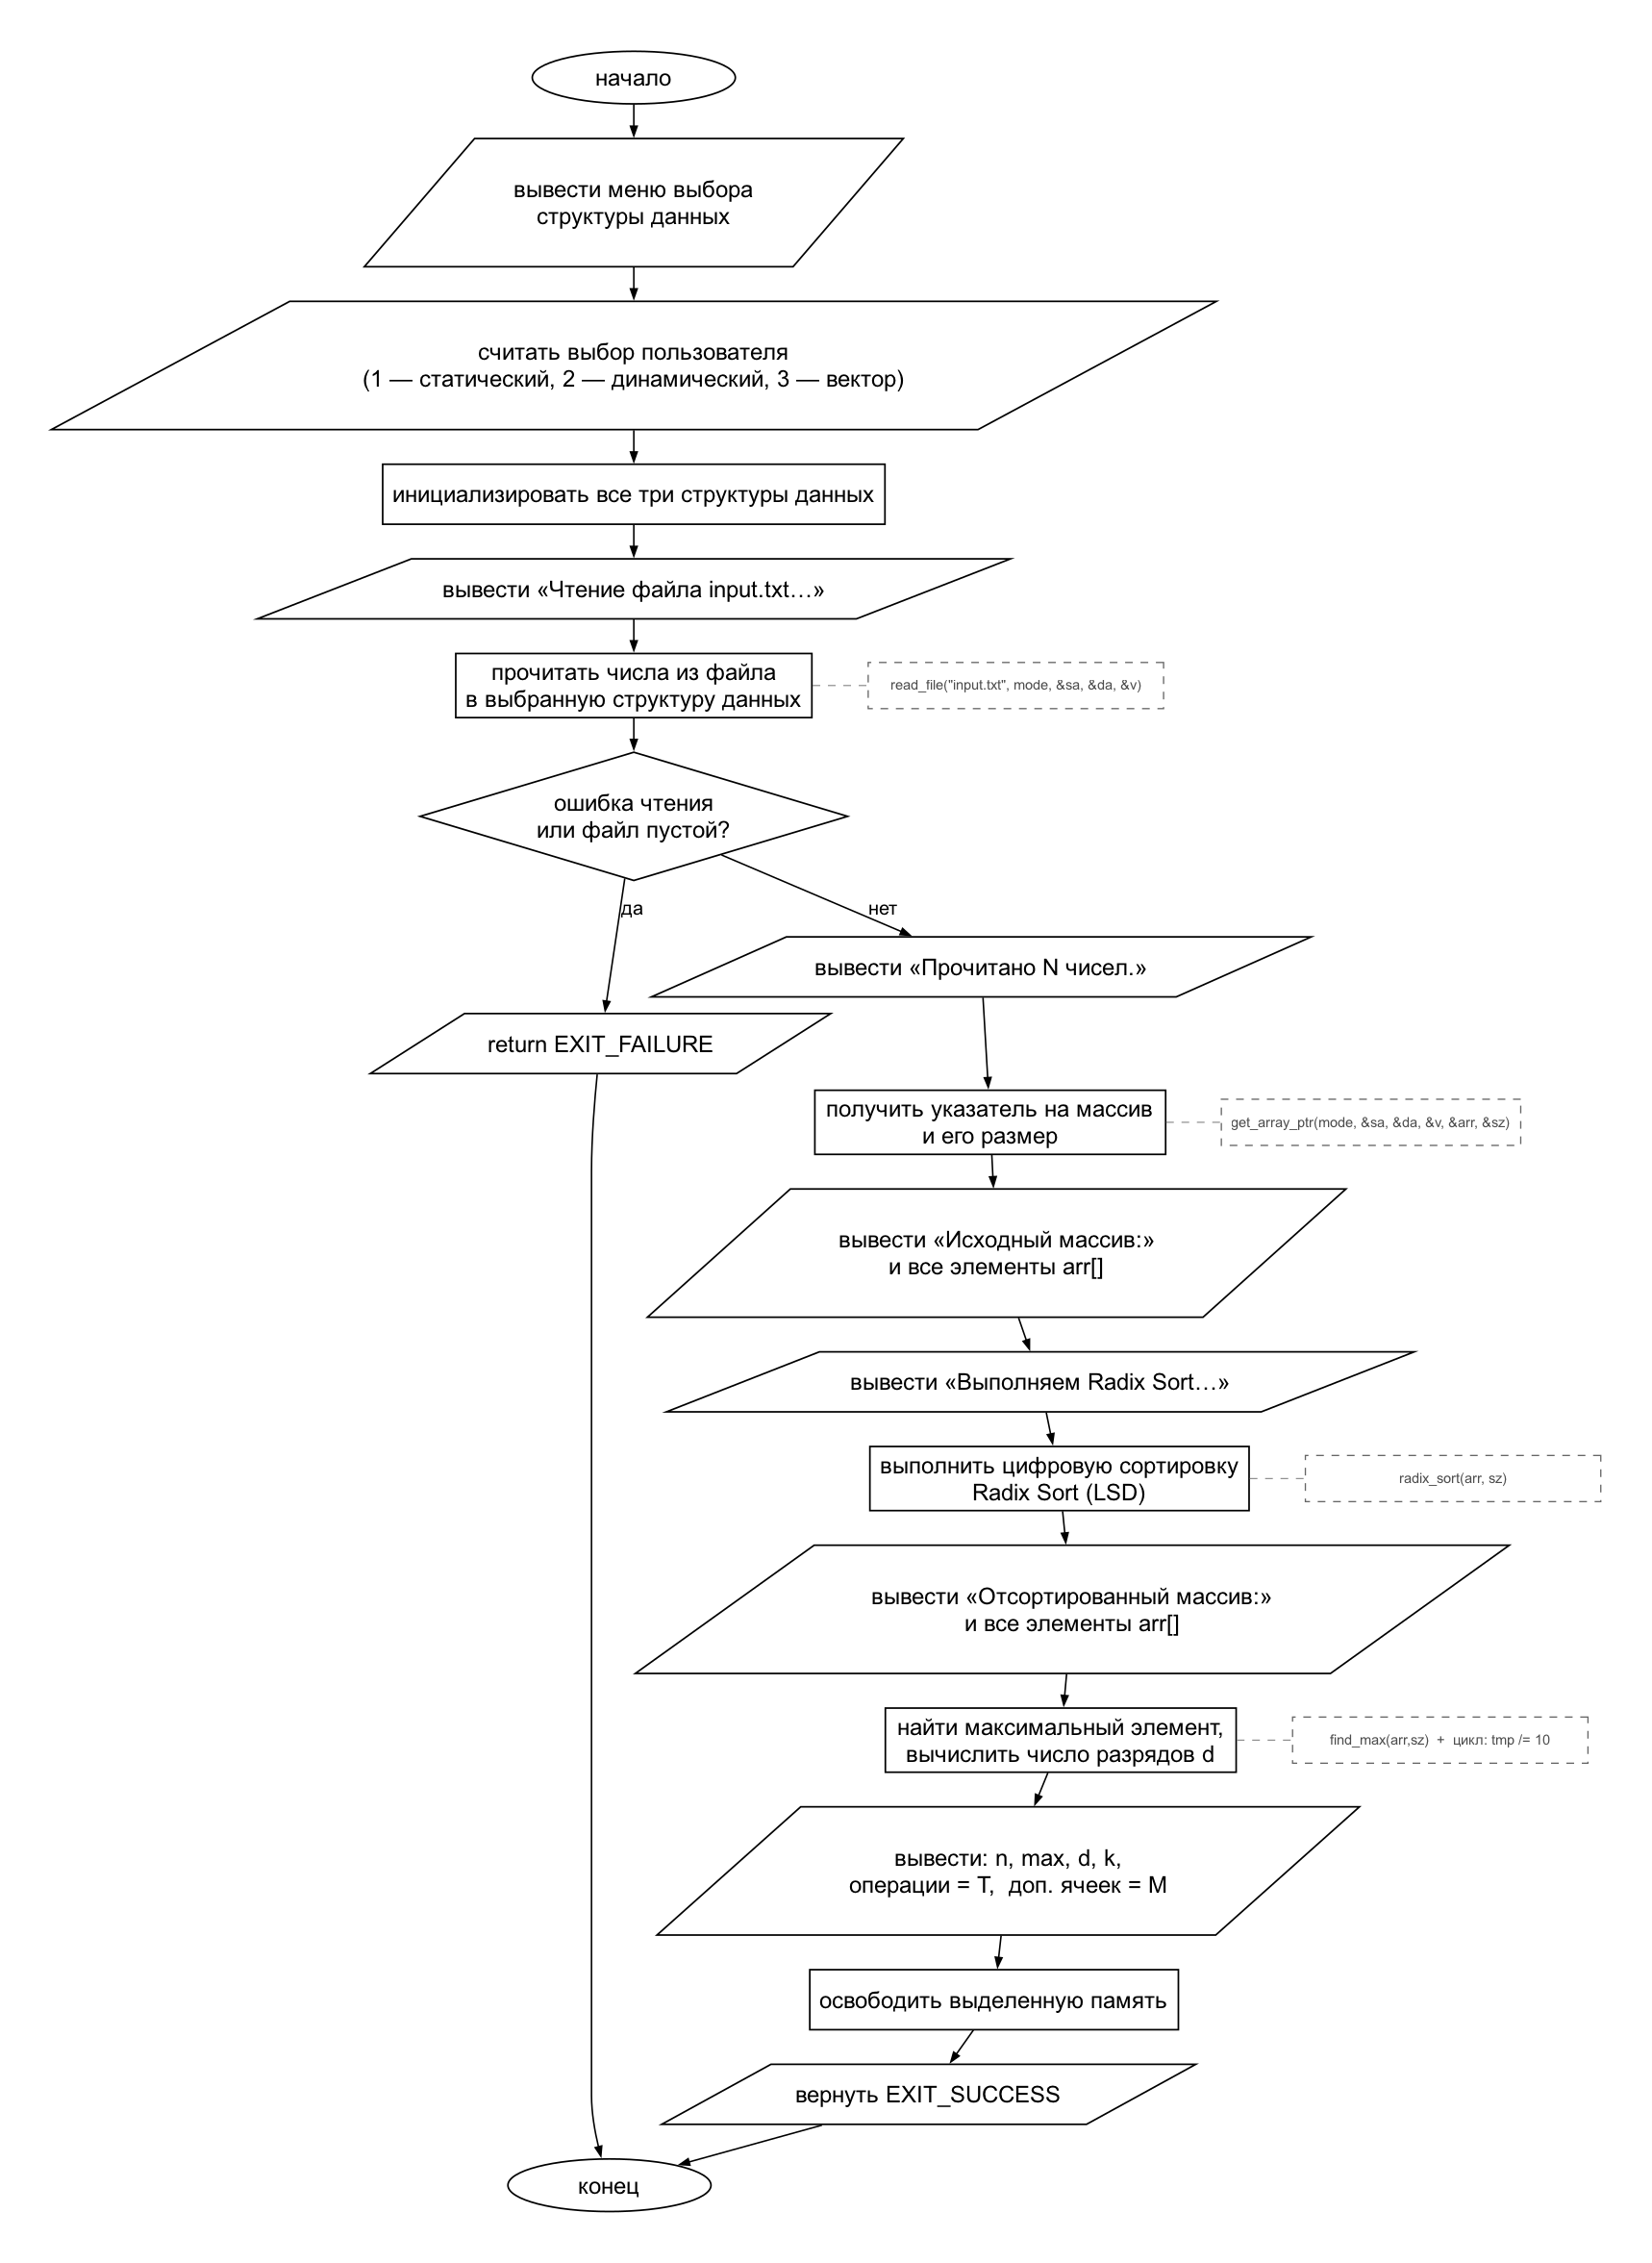
\includegraphics[width=\textwidth,height=0.95\textheight,keepaspectratio]{flowcharts/1_main.png}
\caption{Главная программа (main)}
\end{figure}

\begin{figure}[H]
\renewcommand{\figurename}{Рис.}
\centering
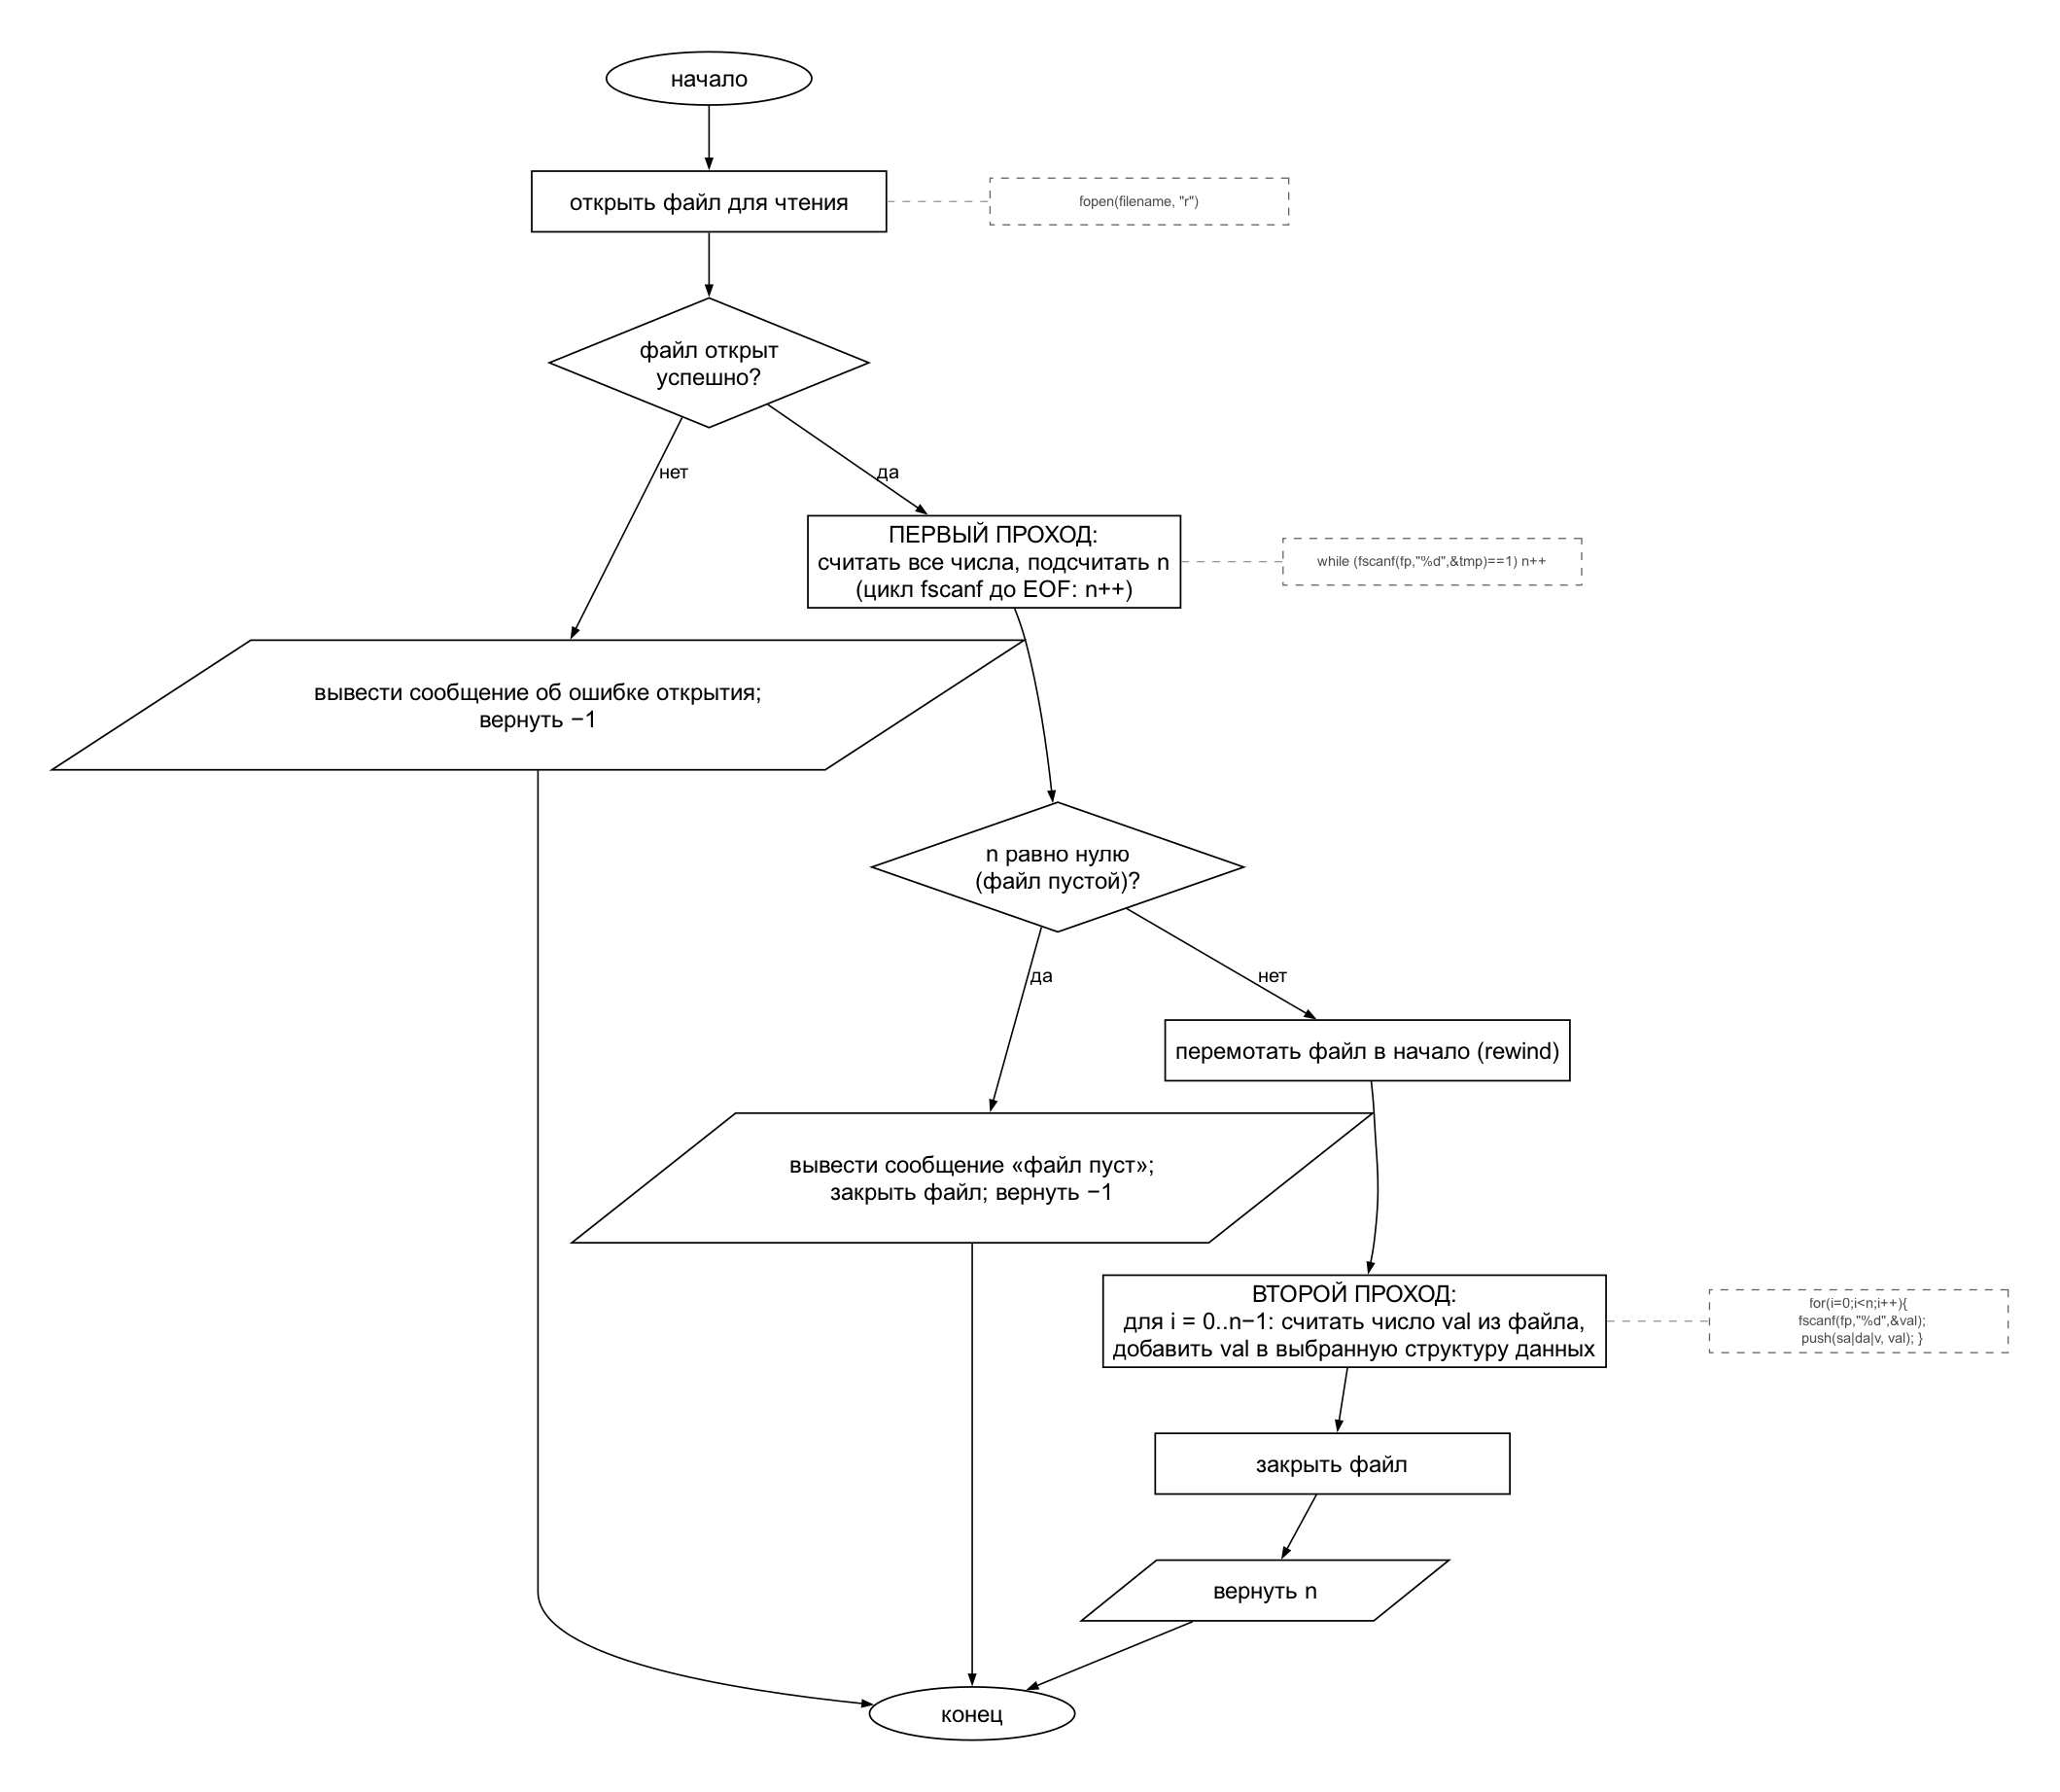
\includegraphics[width=0.85\textwidth]{flowcharts/2_read_file.png}
\caption{Чтение из файла (read\_file)}
\end{figure}

\begin{figure}[H]
\renewcommand{\figurename}{Рис.}
\centering
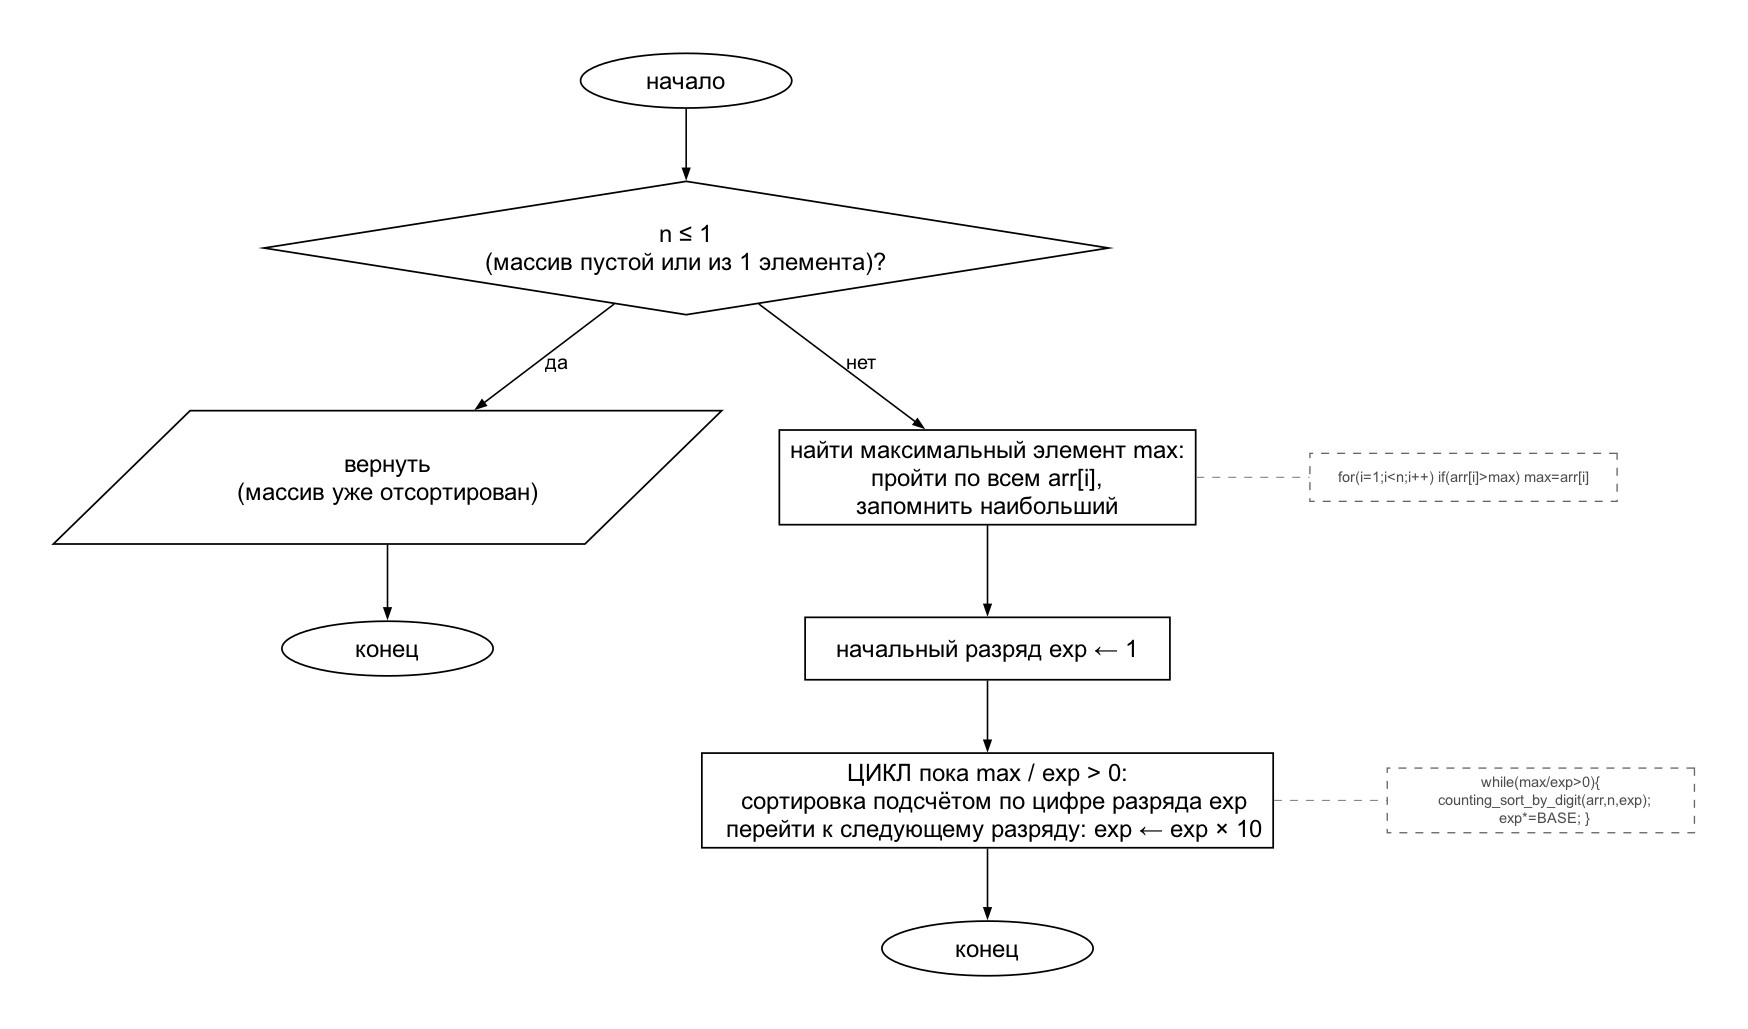
\includegraphics[width=0.75\textwidth]{flowcharts/3_radix_sort.png}
\caption{Цифровая сортировка (radix\_sort)}
\end{figure}

\begin{figure}[H]
\renewcommand{\figurename}{Рис.}
\centering
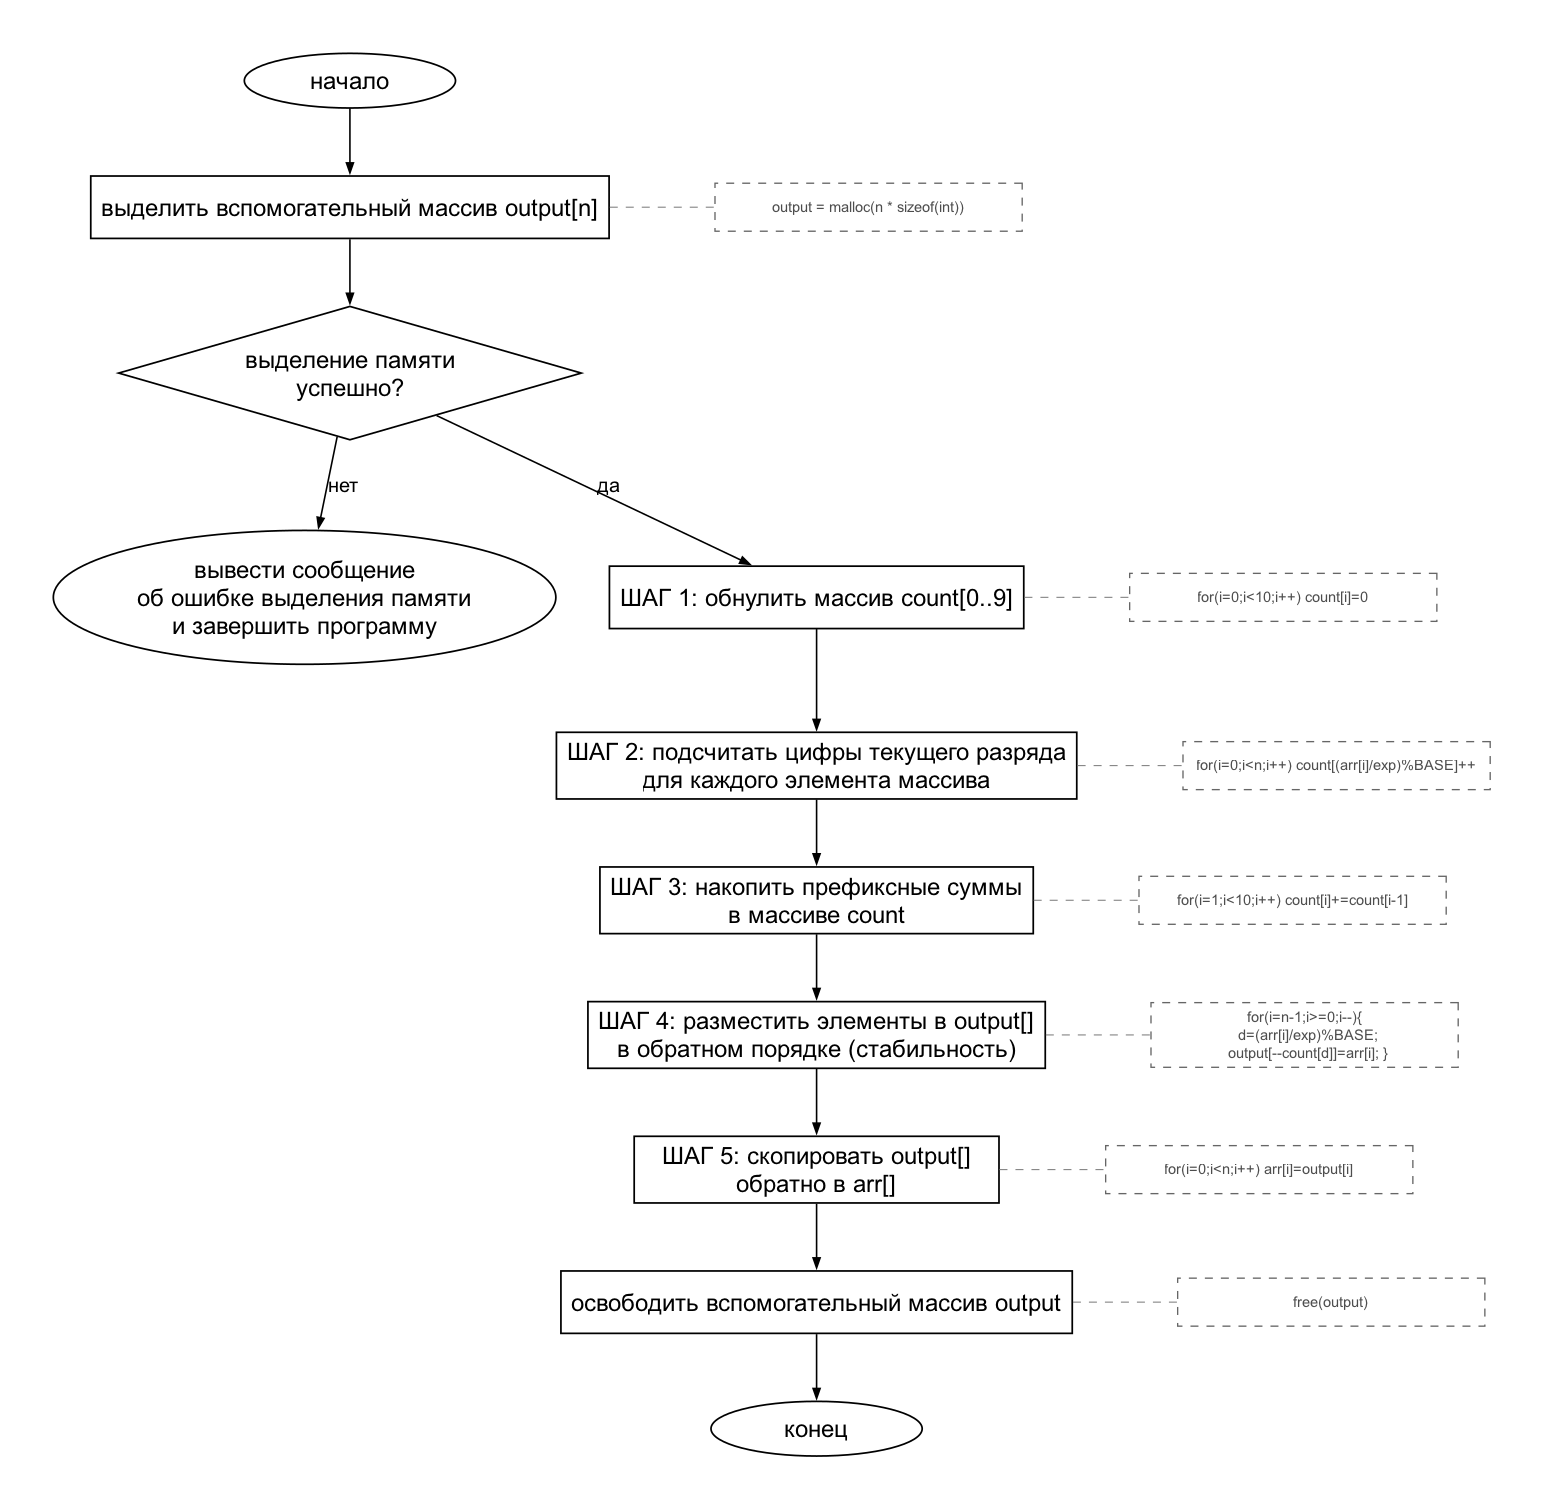
\includegraphics[width=1.0\textwidth]{flowcharts/4_counting_sort.png}
\caption{Сортировка подсчётом по разряду (counting\_sort\_by\_digit)}
\end{figure}

\begin{figure}[H]
\renewcommand{\figurename}{Рис.}
\centering
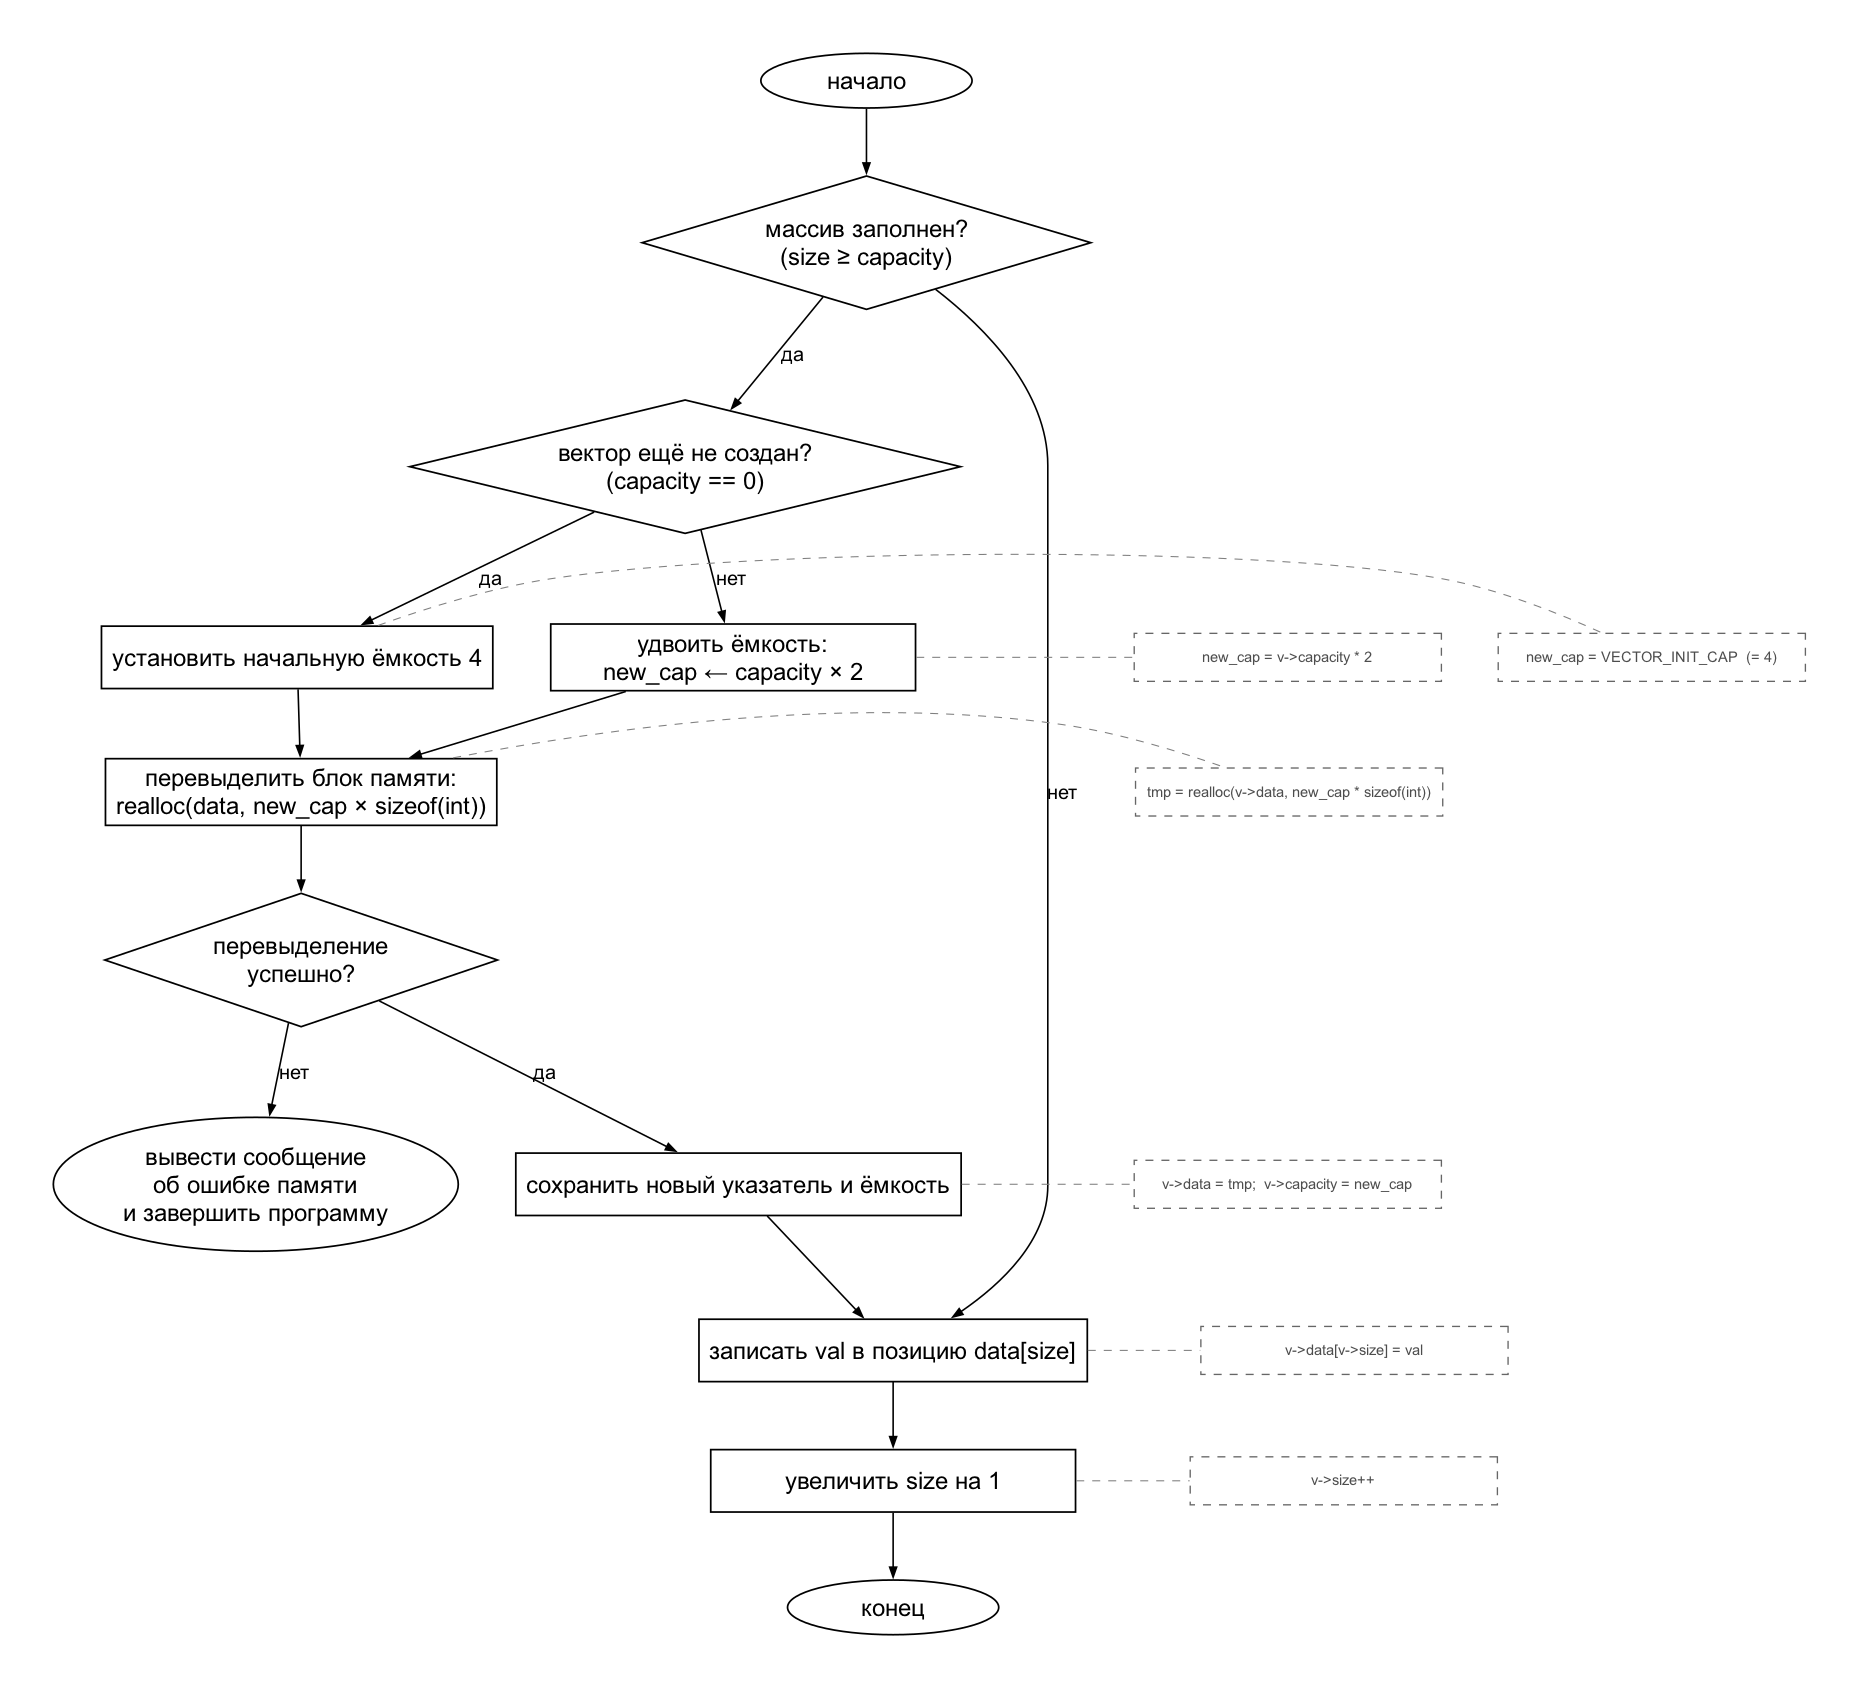
\includegraphics[width=0.85\textwidth]{flowcharts/5_vector_push.png}
\caption{Добавление элемента в вектор (vector\_push)}
\end{figure}

\end{document}
